\documentclass[a4paper]{article}
\usepackage[warn]{mathtext}
\usepackage[utf8]{inputenc}
\usepackage[T2A]{fontenc}

\usepackage[english,russian]{babel}
\usepackage{multicol}
\usepackage{fancyhdr}
\usepackage{graphicx}
\usepackage{microtype}
\usepackage{wrapfig}
\usepackage{amsmath}
\usepackage{floatflt}
\usepackage{geometry} \geometry{verbose,a4paper,tmargin=2cm,bmargin=2cm,lmargin=1.5cm,rmargin=1.5cm}
\usepackage{float}
\usepackage{amssymb}
\usepackage{caption}
\usepackage{epsfig}
\usepackage{newunicodechar}

\begin{document}

\graphicspath{ {pictures/} }

\begin{titlepage}
	\centering
	\vspace{5cm}
    {\scshape\LARGE Московский физико-технический институт\par}
	\vspace{5cm}
	{\scshape\Large Лабораторная работа по общей физике \par}
	\vspace{1cm}
    {\huge\bfseries  6.1 Эффект Мессбауэра \par}
	\vspace{1cm}
	\vfill
    \begin{flushright}
        {\large выполнил студент Б04-852 группы ФЭФМ}\par
        \vspace{0.3cm}
        {\LARGE Яромир Водзяновский}
    \end{flushright}
	\vfill
Долгопрудный, 2021
% Bottom of the page
\end{titlepage}

\pagestyle{fancy} 
\fancyhead[L]{Эффект Мессбауэра    $\sim  \hat(\, ^{\circ}  \omega  ^{\circ} \, \hat) \sim$}
\fancyhead[R]{Современная физика}
\fancyhead[C]{}
\fancyfoot[C]{ \noindent\rule{\textwidth}{0.4pt} \thepage }

\tableofcontents

\newpage



\section{Цель работы}

\begin{itemize}
    \item С помощью метода доплеровского сдвига мессбауэрской линии поглощения исследвуется резонансное поглощение
    $\gamma$-лучей, испускаемых ядрами олова $^{119}Sn$ в соединении $Ba Sn O_3$ при комнатной температуре.
    \item Определить положение максимума резонансного поглощения, его величины, а также экспериментальной ширины линии 
    $\Gamma_{экс}$.
    \item Оценить время жизни возбужденного состояния ядра $^{119}Sn$.
    
\end{itemize}


\section{Теория}

\subsection{Свободные ядра атомов}

Нуклоны в ядре могут находить на разных энергетических уровнях, самый низкий - усновной, а остальные - возбужденные. 
Ядра могут спонтанно переходить на более низкие энергитические уровни, вследстивие появится $\gamma$-излучение. \par 

В отличие от основного уровня, все возбужденные уровни имеют конечную ширину. Если отложим по оси абсцисс энергию ядра, а по оси ординат - 
вероятность найти ядро в состоянии с данной жнергии, то ширина кривой, измеренная на половине высоты, называется шириной линии $\Gamma$ и она 
связана со средним временем жизни $\tau$ возбужденного состояния:

\begin{equation}
    \Gamma \cdot \tau \approx \hbar 
\end{equation}

\begin{wrapfigure}[16]{l}{130pt}
    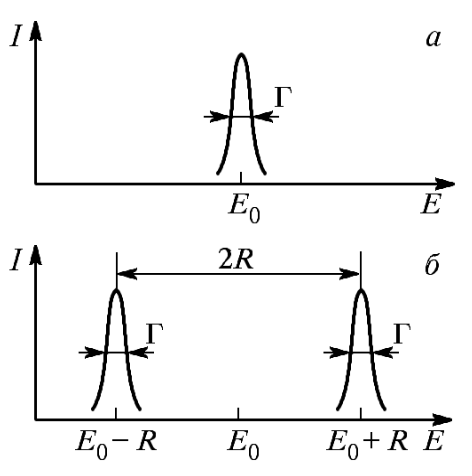
\includegraphics[scale = 0.5]{p1.png}
    \caption{Энергетическое распределение, характеризующее возбужденное состояние (а), и с двиг линий испускания и поглощения из-за отдачи.}
    \label{p1}
\end{wrapfigure}

Ядро также может поглотить фотон и перейти на более высокое состояние если энергия фотона равна разности энергий между состояниями.
Этот процесс носит резонансный характер. \par 

Не так просто обнаружить этот эффект, т.к. энергия $E_{\gamma}$, уносимая $\gamma$-квантом, оказывается меньше энергии $E_0$ перехода между уровнями.
Также часть энергии уносится ядром, вследствие отдачи оно начинает двигаться в противоположную $\gamma$-кванту сторону. \par 

По ЗСИ ядро получит импульс равный импульсу фотона, тогда энергия отдачи $R$:
\begin{equation}
    R = \frac{p^2}{M_{я}} = \frac{E_{\gamma}^2}{2 M_{я} c^2}
\end{equation}

Для олова $E_0 = 23.8\; кэВ$, $R \approx 2.5 \cdot 10^{-3} \; эВ$. На рис. \ref{p1} видно, как сдвигается 
линия поглощения вправо, а испускания - влево. 

Резонансное поглощение возможно если спектры испускания и поглощения перекрываются:

ЯЯЯЯЯЯРириккк

\begin{equation}
    2R \leq \Gamma
\end{equation}

Однако это условие почти никогда не выполняется для $\gamma$-переходов в свободных ядрах. 

Можно компенсировать энергетический сдвиг с помощь/ эффекта Доплера. Для этого будем двигать излучаюшие 
и поглощающие ядра относительно друг друга со скоростью:

\begin{equation}
    V = c \cdot 2R / E_{\gamma} \approx 60 \; м/с
\end{equation}

\begin{wrapfigure}[13]{l}{130pt}
    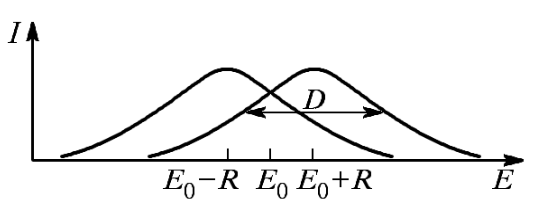
\includegraphics[scale = 0.5]{p2.png}
    \caption{Перекрытие линий испускания и поглощения вследствие доплеровского сдвига}
    \label{p2}
\end{wrapfigure}

Ширина линии складывается из собственной и доплеровской ширины, основную роль играет доплеровская, связанная с тепловым движением атомов.
Доплеровский сдвиг:

\begin{equation}
    D = 2 \sqrt{R k_Б T} \approx 1.5 \cdot 10^{-2} \; эВ
\end{equation}

Доплеровская ширина оказывается больше собтсвенной и больше сдвига R. В результате доплеровског уширения 
частично линии будут перекрываться (рис. \ref{p2}) и будет доля $\gamma$-квантов, для которыз отдача R скомапенсирована и возможно резонансное 
поглощение. 

\

\subsection{Ядра атомов в кристаллической решетке}

Энергия, необходимая для смещения ядра $10 \div 30 \;  эВ$. При испускании $\gamma$-квантов с $E < 1 \; МэВ$ энергия отдачи 
недостаточна для вырывания ядра из кристаллической решетки, энергия отдачи переходит в звуковые колебания, переносимые фононами. 
Процесс генерации фононов тем легче, чем их больше, то есть при больших температурах. В формуле (2) вместо массы ядра будет масса всего кристалла и 
энергия отдачи понизиться на $10 \div 20 $ порядков и становится очень малой. \par 

\textbf{Эффект Мессбауэра} - испускание и поглощение $\gamma$-квантов в твердых телах без рождения фононов.

Вероятность эффекта оценивается выражением:

\begin{equation}
    f = e^{-4 \pi^2 \langle u^2 \rangle / \lambda^2}
\end{equation}

$\langle u^2 \rangle$ - среднеквадратичное смещение ядер в процессе тепловых колебаний решетки (в направлении вылеты $\gamma$-кванта), 
$\lambda$ - длина волны излучения. Видно, что вероятность уменьшается с ростом температуры и растет с уменьшением длины волны. \par 

Эффект Мессбауэра ограничен областью малых энергий $\gamma$-лучей $\approx 200 \; кэВ$. Линия резонансного мессбауэрского поглощения 
не размыта тепловым движением и имеет малую ширину. \par 

Отсутсвие доплеровского уширения из-за беспорядочноо теплового движения атомов связано с тем, что частота тепловых колебаний много больше, чем 
частота жизни мессбауэрских ядерных уровней, поэтому за время испускания $\gamma$-кванта ядро успевает много раз сменить направение скорости и 
среднее значени равно нулю. \par 

Гамма излучение пропускается через резонансный поглотитель, где находятся ядра $^{119}Sn$, тут происзодит взаимодествие квантов с электронами за счет фотоэффекта и эффекта Комптона и взаимодействие с ядрами. 
Интенсивность проходящего через поглотитель излучения уменьшается как:

\begin{equation}
    e^{-n_e \sigma_e} e^{-n f \sigma(E)}
\end{equation}

$n_e, \;\; n$ - число электронов и ядер поглотителя на $1 \; см^2$ поглотителя, $f$ - вероятность Мессбауэра, $\sigma_e, \;\; \sigma(E)$ - 
сечение взаимодействия с электронами среды и сечение резонансного поглощения. Сечения резонансного поглощения имеет вид лоренца:

\begin{equation}
    \sigma(E) \propto \frac{(\Gamma/2)^2}{(E - E_0)^2 + (\Gamma/2)^2}
\end{equation}


$E_0$ - энергия ядерного перехода, $\Gamma$ - естественная ширина линии. Излучение, прошедшее через поглотитель, регистрируется сцинтилляционным спектрометром. \par 

Наблюдать резонансное поглощение будем используя метод доплеровского сдвига, для создания которого поглатителю будет сообщена скорость порядка миллиметра в секунду. 

Ядра источника и поглотителя находятся в идентичных кристаллах при одной температуре, то их линии полностью перекрываются и максимум поглощения при нулевой скорости (рис. ref{p3})

\begin{figure}
    \begin{center}
        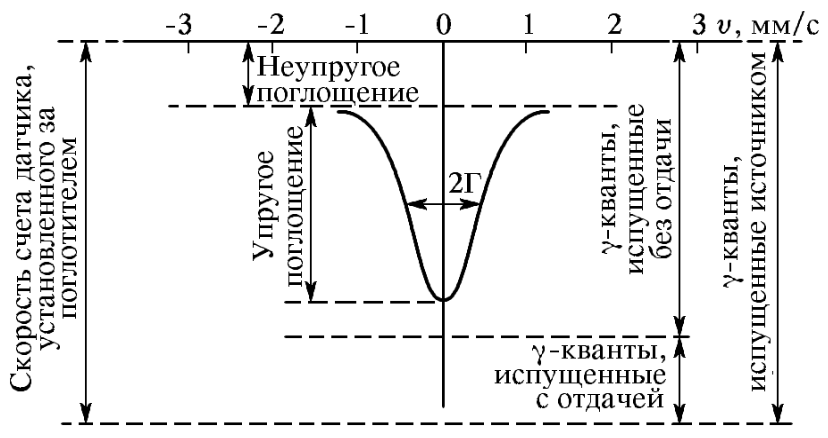
\includegraphics[scale = 0.5]{p3.png}
        \caption{Спектр упругого резонансного поглощения $\gamma$-квантов.}
        \label{p3}
    \end{center}
\end{figure}

Если ядра входят в состав химических соединений, то максимум линии поглощения будет наблюдаться при ненулевой скорости.
Т к энергия ядерного перехода зависит от электростатических сил взаимодействия ядра с окружающими электронами, что сравнительно с шириной линии упругого 
резонансного поглощения. Смещение максимума линии легко замечается и называется химическим сдвигом. \par 

Для источника и поглотителя из разынх хим. соединений смещение максимума по скорости:

\begin{equation}
    v_p = \frac{\Delta E}{E_0} c
\end{equation}

Величина амплитуды эффекта:

\begin{equation}
    \varepsilon (v) = \frac{N(\infty) - N(v)}{N(\infty) - N_ф}
\end{equation}

$N(v)$ - скорость счета квантовб прошедших через поглотитель при скорости $v$, $N(\infty)$ - скорость счета квантов при достаточно большой скорости, когда резонансное поглощение отсутсвиествует,
$N_ф$ - скорость счета радиоактивного фона. \par 

На опыте измеренная $\Gamma_{эксп}$ - результат наложения линий источника и поглотителя, в идеальных условиях ширина линии равна удвоенной естественной ширине $2 \Gamma$.
Увеличение толщины поглотителя заметно уширяет резонансную линию, тк:

\begin{itemize}
    \item Кванты, энергия которых вблизи максимума линии уже сильно поглощаются в тонких и ширина почти не имеет значения.
    \item Уширение лини может происходить и вследствие самопоглощения квантов в источнике.
    \item Аппаратурное уширение - вибрации источника
    \item Неравномерность скорости перемещения поглотителя
\end{itemize}


\section{Экспериментальаня установка}

\begin{figure}[H]
    \begin{center}
        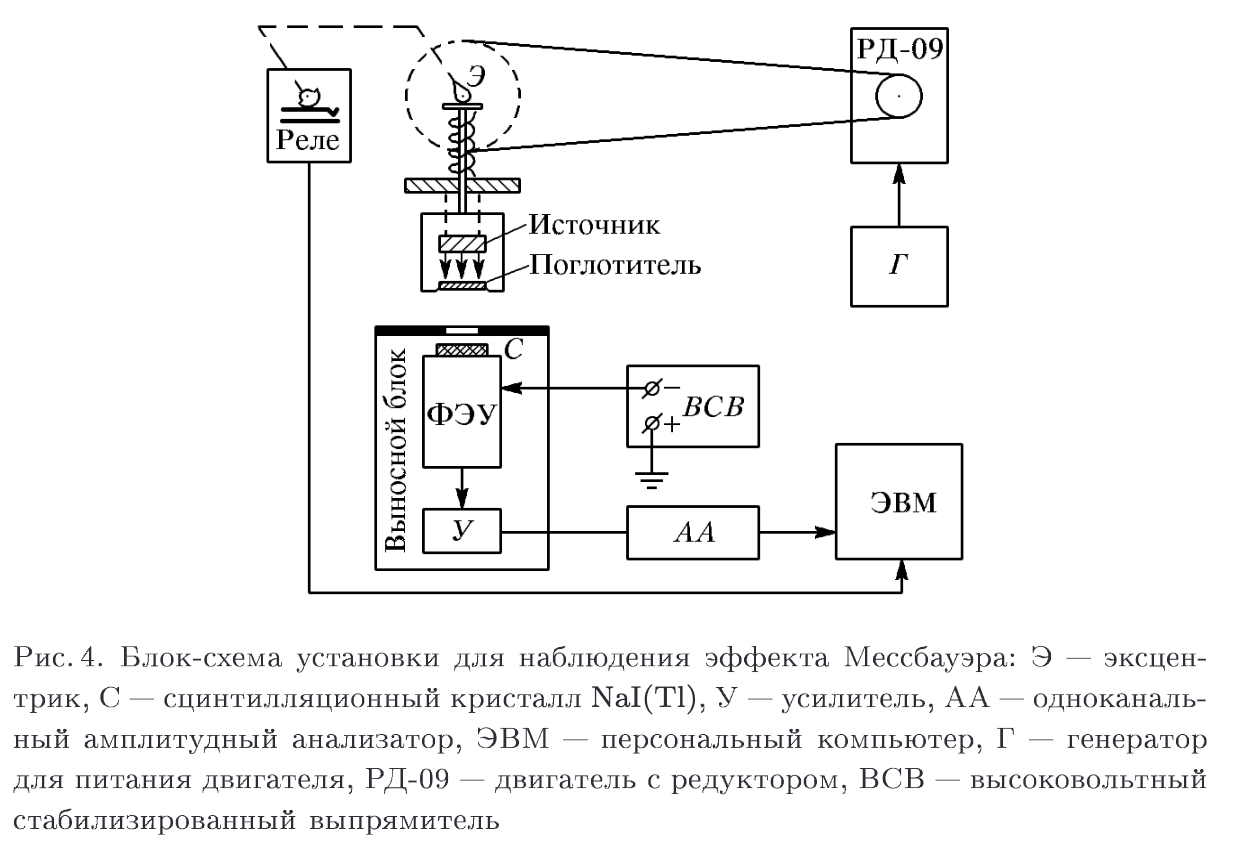
\includegraphics[scale = 0.5]{setup.png}
        \caption{}
        \label{setup}
    \end{center}
\end{figure}

В работе используется источник $\gamma$-квантов радиоактивный изотоп олова $^{119m}Sn$ в 
виде соединения $BaSnO_3$, распадается с излучением гамма-квантов $\approx 65\; кэВ$, переходя 
на первый возбужденный уровень (рис. \ref{p4}). При переходе с первого уровня на основной излучается $\gamma$-квант 
$23.8 \; кэВ$. 


\begin{figure}[h]
    \begin{center}
        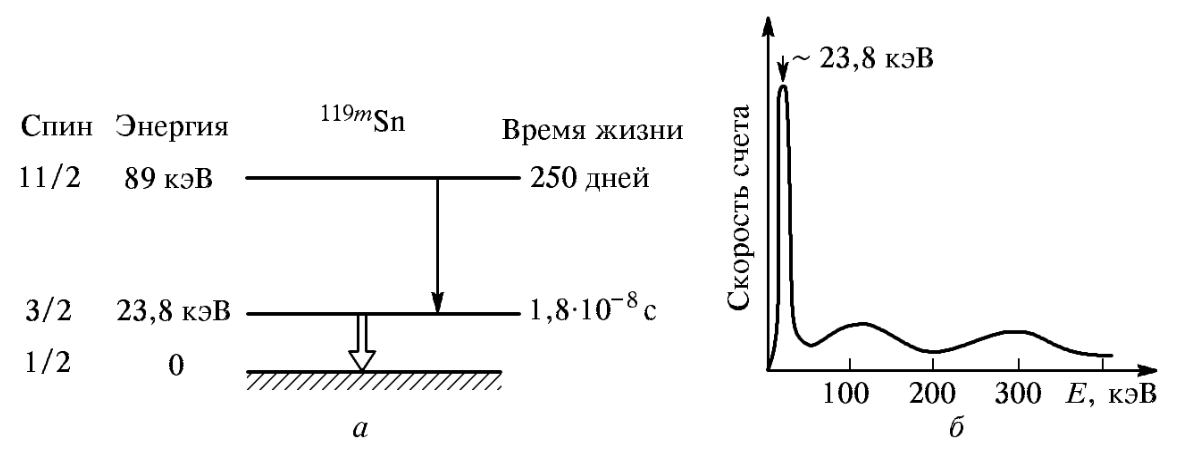
\includegraphics[scale = 0.5]{p4.png}
        \caption{Схема распада $^{119}Sn$ (а) ; спектр излучения источника $BaSnO_3$}
        \label{p4}
    \end{center}
\end{figure}

На рис. \ref{p4}б, показан спектр излучения источника. Видны также размытые пики на 100 кэВ и 300 кэВ. Для наблюдения эффекта 
нужно выделить основную линию из общего излучения, установив окно амплитудного анализатора. 


\section{Ход работы}

\subsection{Измерение спектра источника и его анализ}

\textit{Цель - подобрать настройки анализатора импульса так, чтобы детектировались только $\gamma$-кванты с энергией $23.8$ кэВ, исходящие от источника}

\begin{enumerate}
    \item Включим установку, все настроим. Установим ширину окна
    \item Установим ширину окна 0.5 В
    \item Измерим интенсивность излучения (скорость счета) двигая окно от 0 до 9.5 В
    \item Результат занесем в таблицу 1 и нанесем на график (рис. \ref{N(V)})
    \item Сделаем фит функцией Лоренца (Распределение Коши):
    
    \begin{equation}
        f(x) = \frac{1}{\pi \gamma \left( 1 + \left(\frac{x - x_0}{\gamma} \right)^2 \right)}
    \end{equation}

    Но в нашем случае немног модернезируем его, чтомы можно было сделать фит:

    \begin{equation}
        f(x) = b  - \frac{a}{1 + \left( \frac{x-d}{c/ \alpha} \right)^2}
    \end{equation}

    Где $\alpha$ - некий коэффициент определяющий вместе с коэффициентом $c$ полуширину на полувысоте, $\alpha$ подбирается каждый раз исходя из прикидывания полуширины, чтобы помочь алгоритму подобрать коэффициенты.
    В итоге $2 \cdot c/\alpha = \Gamma_{экс}$.
    Коэффициент $b$ определяет высоту аппроксимационной кривой. $d$ - есть химический сдвиг. 

\begin{table}[H]
    \centering
    \caption{}
    \label{t1}
    \vspace{0.1cm}
    \begin{tabular}{|c||c|c|c|c|c|c|c|c|c|c|c|c|c|c|c|c|c|c|}
 \hline
N, $c^{-1}$ & 674.6&270&386&919.3&1982.7&3375.3&4593.1&4787.1&3833.1&2405.3\\
\hline
U, В & 0.5 & 1 & 1.5 & 2 & 2.5  & 3 & 3.5 & 4&4.5&5   \\
\hline
\hline
N, $c^{-1}$ & 1205.9&538.4&215.8&109.4&79.8&55.9&46.4&36.6&29.7& \\ 
\hline
U, В & 5.5&6&6.5&7&7.5&8&8.5&9&9.5& \\
\hline
\end{tabular}
\end{table}

\begin{figure}[h]
    \begin{center}
        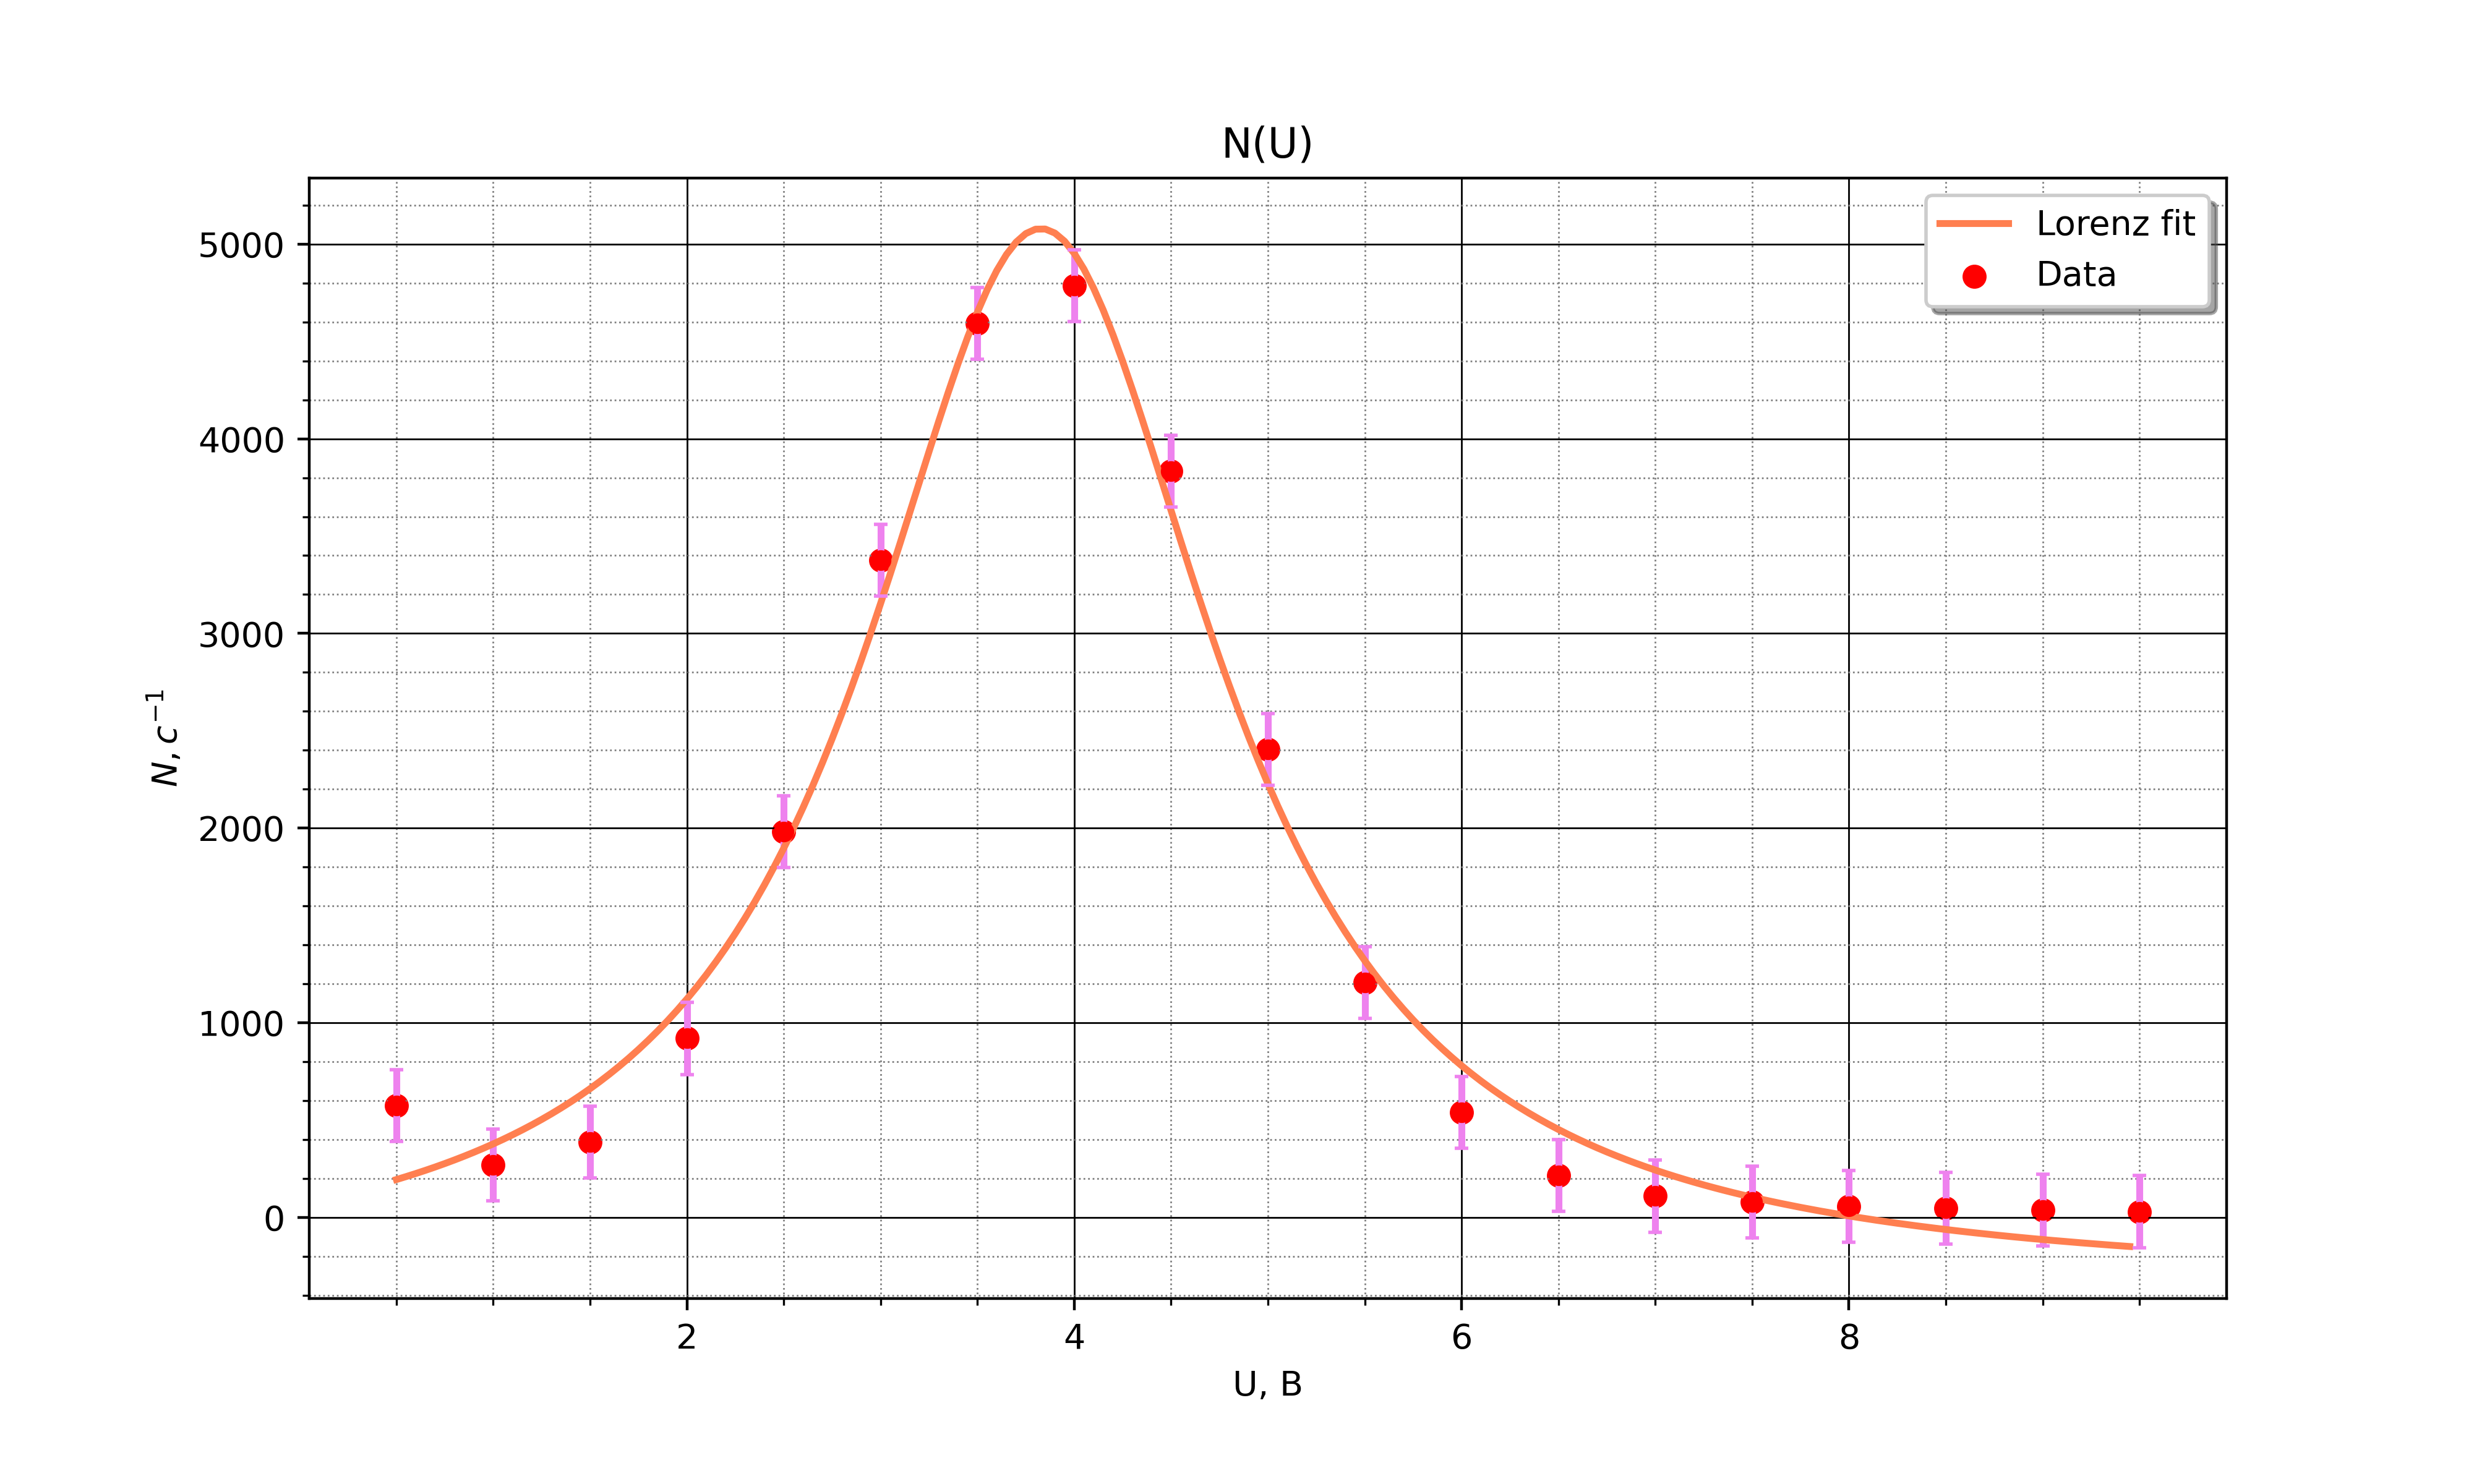
\includegraphics[scale = 0.5]{N(V).png}
        \caption{Измеренный спектр источника}
        \label{N(V)}
    \end{center}
\end{figure}

\item По графику понимаем, что большгая часть нужных нам квантов лежит в диапазоне от 2 до 6 В.

\end{enumerate}


\subsection{Измерение резонансного поглощения}

\textit{Цель - измерить резонансное поглощение для 4х образцов}

\begin{enumerate}
    \item Время измерения 20 секунд.
    \item Измерим фон = 14 1/с
    \item Занесем в таблиуц 2 параметры фитов:
    
    \begin{table}[H]
        \centering
        \caption{}
        \label{t2}
        \vspace{0.1cm}
        \begin{tabular}{|c|c|c|c|c|c|c|c|c|c|}
    \hline
    Поглотитель & a& $\sigma_a$, \% &b, $с^{-1}$& $\sigma_b$, \% & c, мм/с & $\sigma_c$, \% & d, мм/с & $\sigma_d$, \% & $\alpha$ \\ \hline
    1 &-3138.14 & 7.54 & 40332.52 & 0.25 & -1.46 & 14.99 & 2.366 & 2.49 & 2 \\ \hline
    2 & -3304.33 &2.94 &20085.86 & 0.19 & 0.32 & 5.50 &2.31 & 0.84&0.5 \\ \hline
    3 & -1873.44& 4.89& 8715.93& 0.38 & 1.67&7.59 &2.40 &5.27 & 2\\ \hline
    4 &-12250.20 & 1.34& 32588.94& 0.06 & 0.92& 1.42&-0.02 & 13.77&1 \\   \hline
    \end{tabular}
    \end{table}


    \item По полученным параметрам аппроксимации определим следующие величины (таблица 3):
    
    \begin{table}[H]
        \centering
        \caption{}
        \label{t3}
        \vspace{0.1cm}
        \begin{tabular}{|c|c|c|c|c|}
    \hline
    Поглотитель & Хим сдвиг, мм/с& Хим сдвиг, эВ& $\Gamma_{эксп}$, мм/с & $\Gamma_{эксп}$, эВ \\ \hline
    1 & 2.366 & 1.87 $\cdot 10^{-7}$& 1.46 & 1.16 $\cdot 10^{-7}$\\ \hline
    2 & 2.31&  1.83 $\cdot 10^{-7}$ & 1.28& 1.05 $\cdot 10^{-7}$ \\ \hline
    3 & 2.40& 1.9 $\cdot 10^{-7}$&1.67 & 1.32 $\cdot 10^{-7}$ \\ \hline
    4 & -0.02&  1.58 $\cdot 10^{-9}$&0.04& 3.17 $\cdot 10^{-9}$\\   \hline
    \end{tabular}
    \end{table}

    Величина зимического сдвига в эВ:

    \begin{equation}
        \Delta E = E \frac{v}{c}
    \end{equation}

    $E = 23.8\; кэВ$ \par 

    Экспериментальная ширина линии $\Gamma_{эксп}$ в эВ:

    \begin{equation}
        \Gamma_{эксп} = 2\Gamma = E \frac{v}{c}
    \end{equation}



\end{enumerate}

\begin{figure}[H]
    \begin{center}
        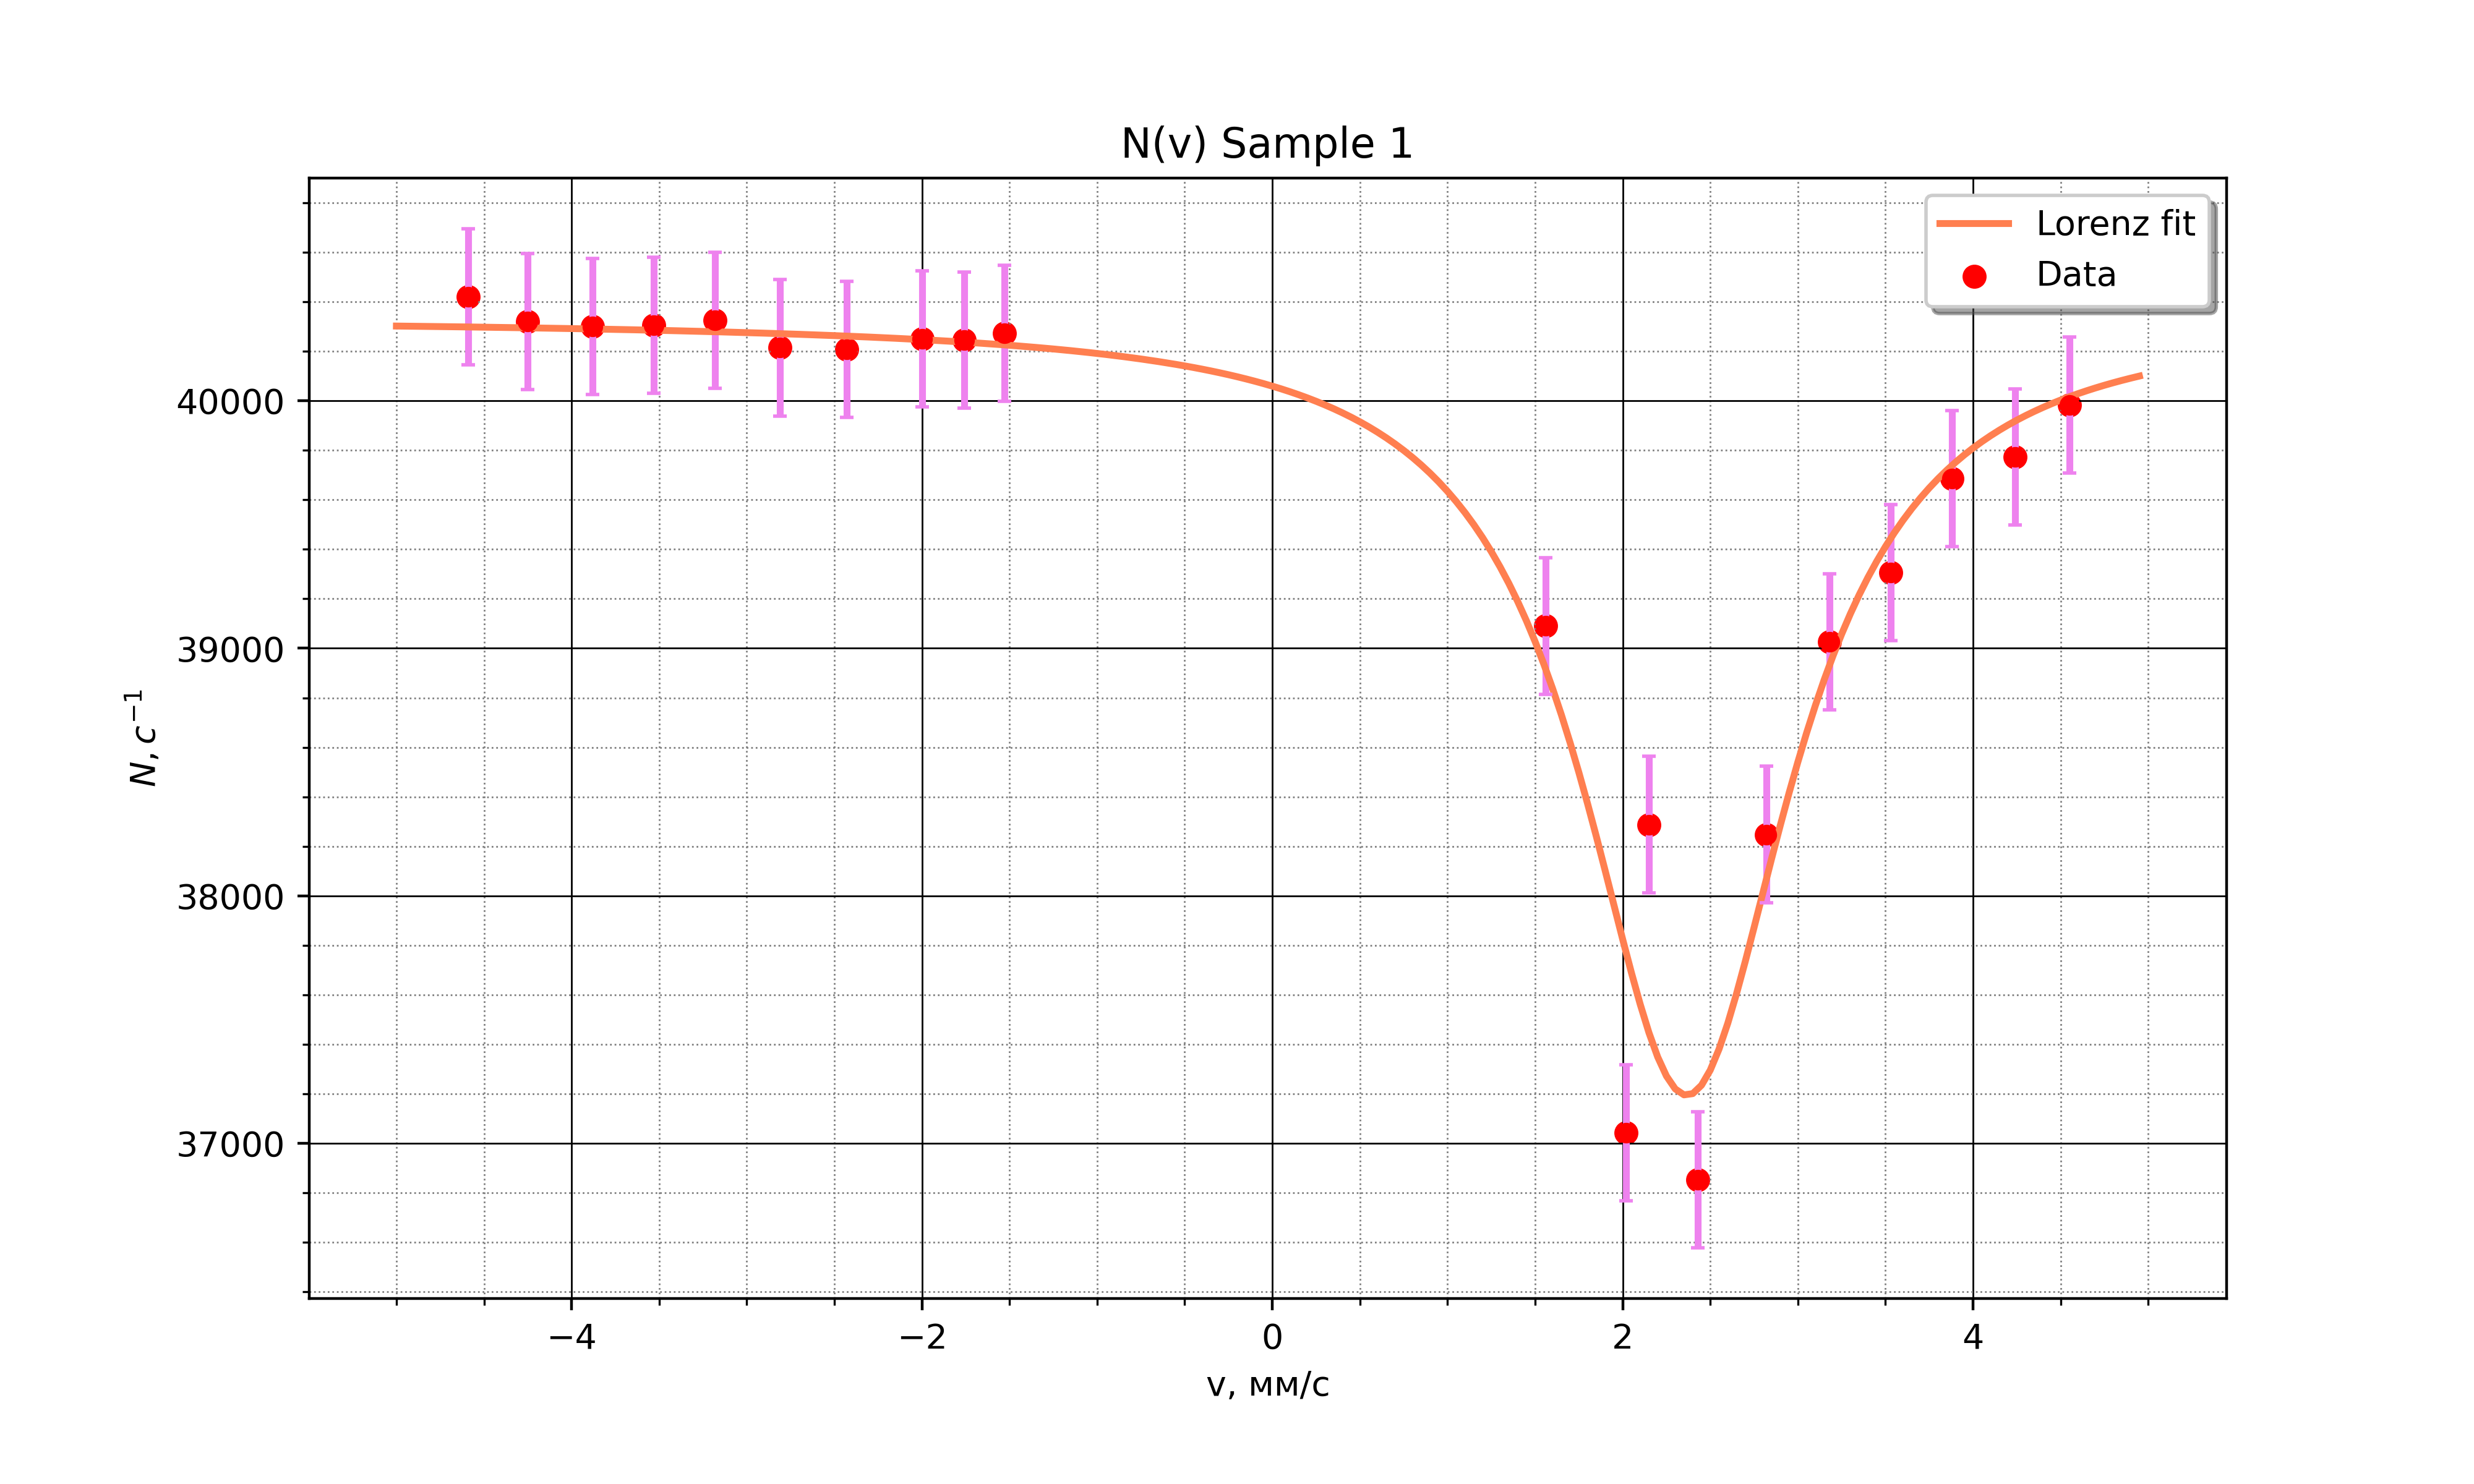
\includegraphics[scale = 0.5]{S1fit.png}
        \caption{Резонансное поглощение на 1-м образце}
        \label{S1fit}
    \end{center}
\end{figure}

\begin{figure}[H]
    \begin{center}
        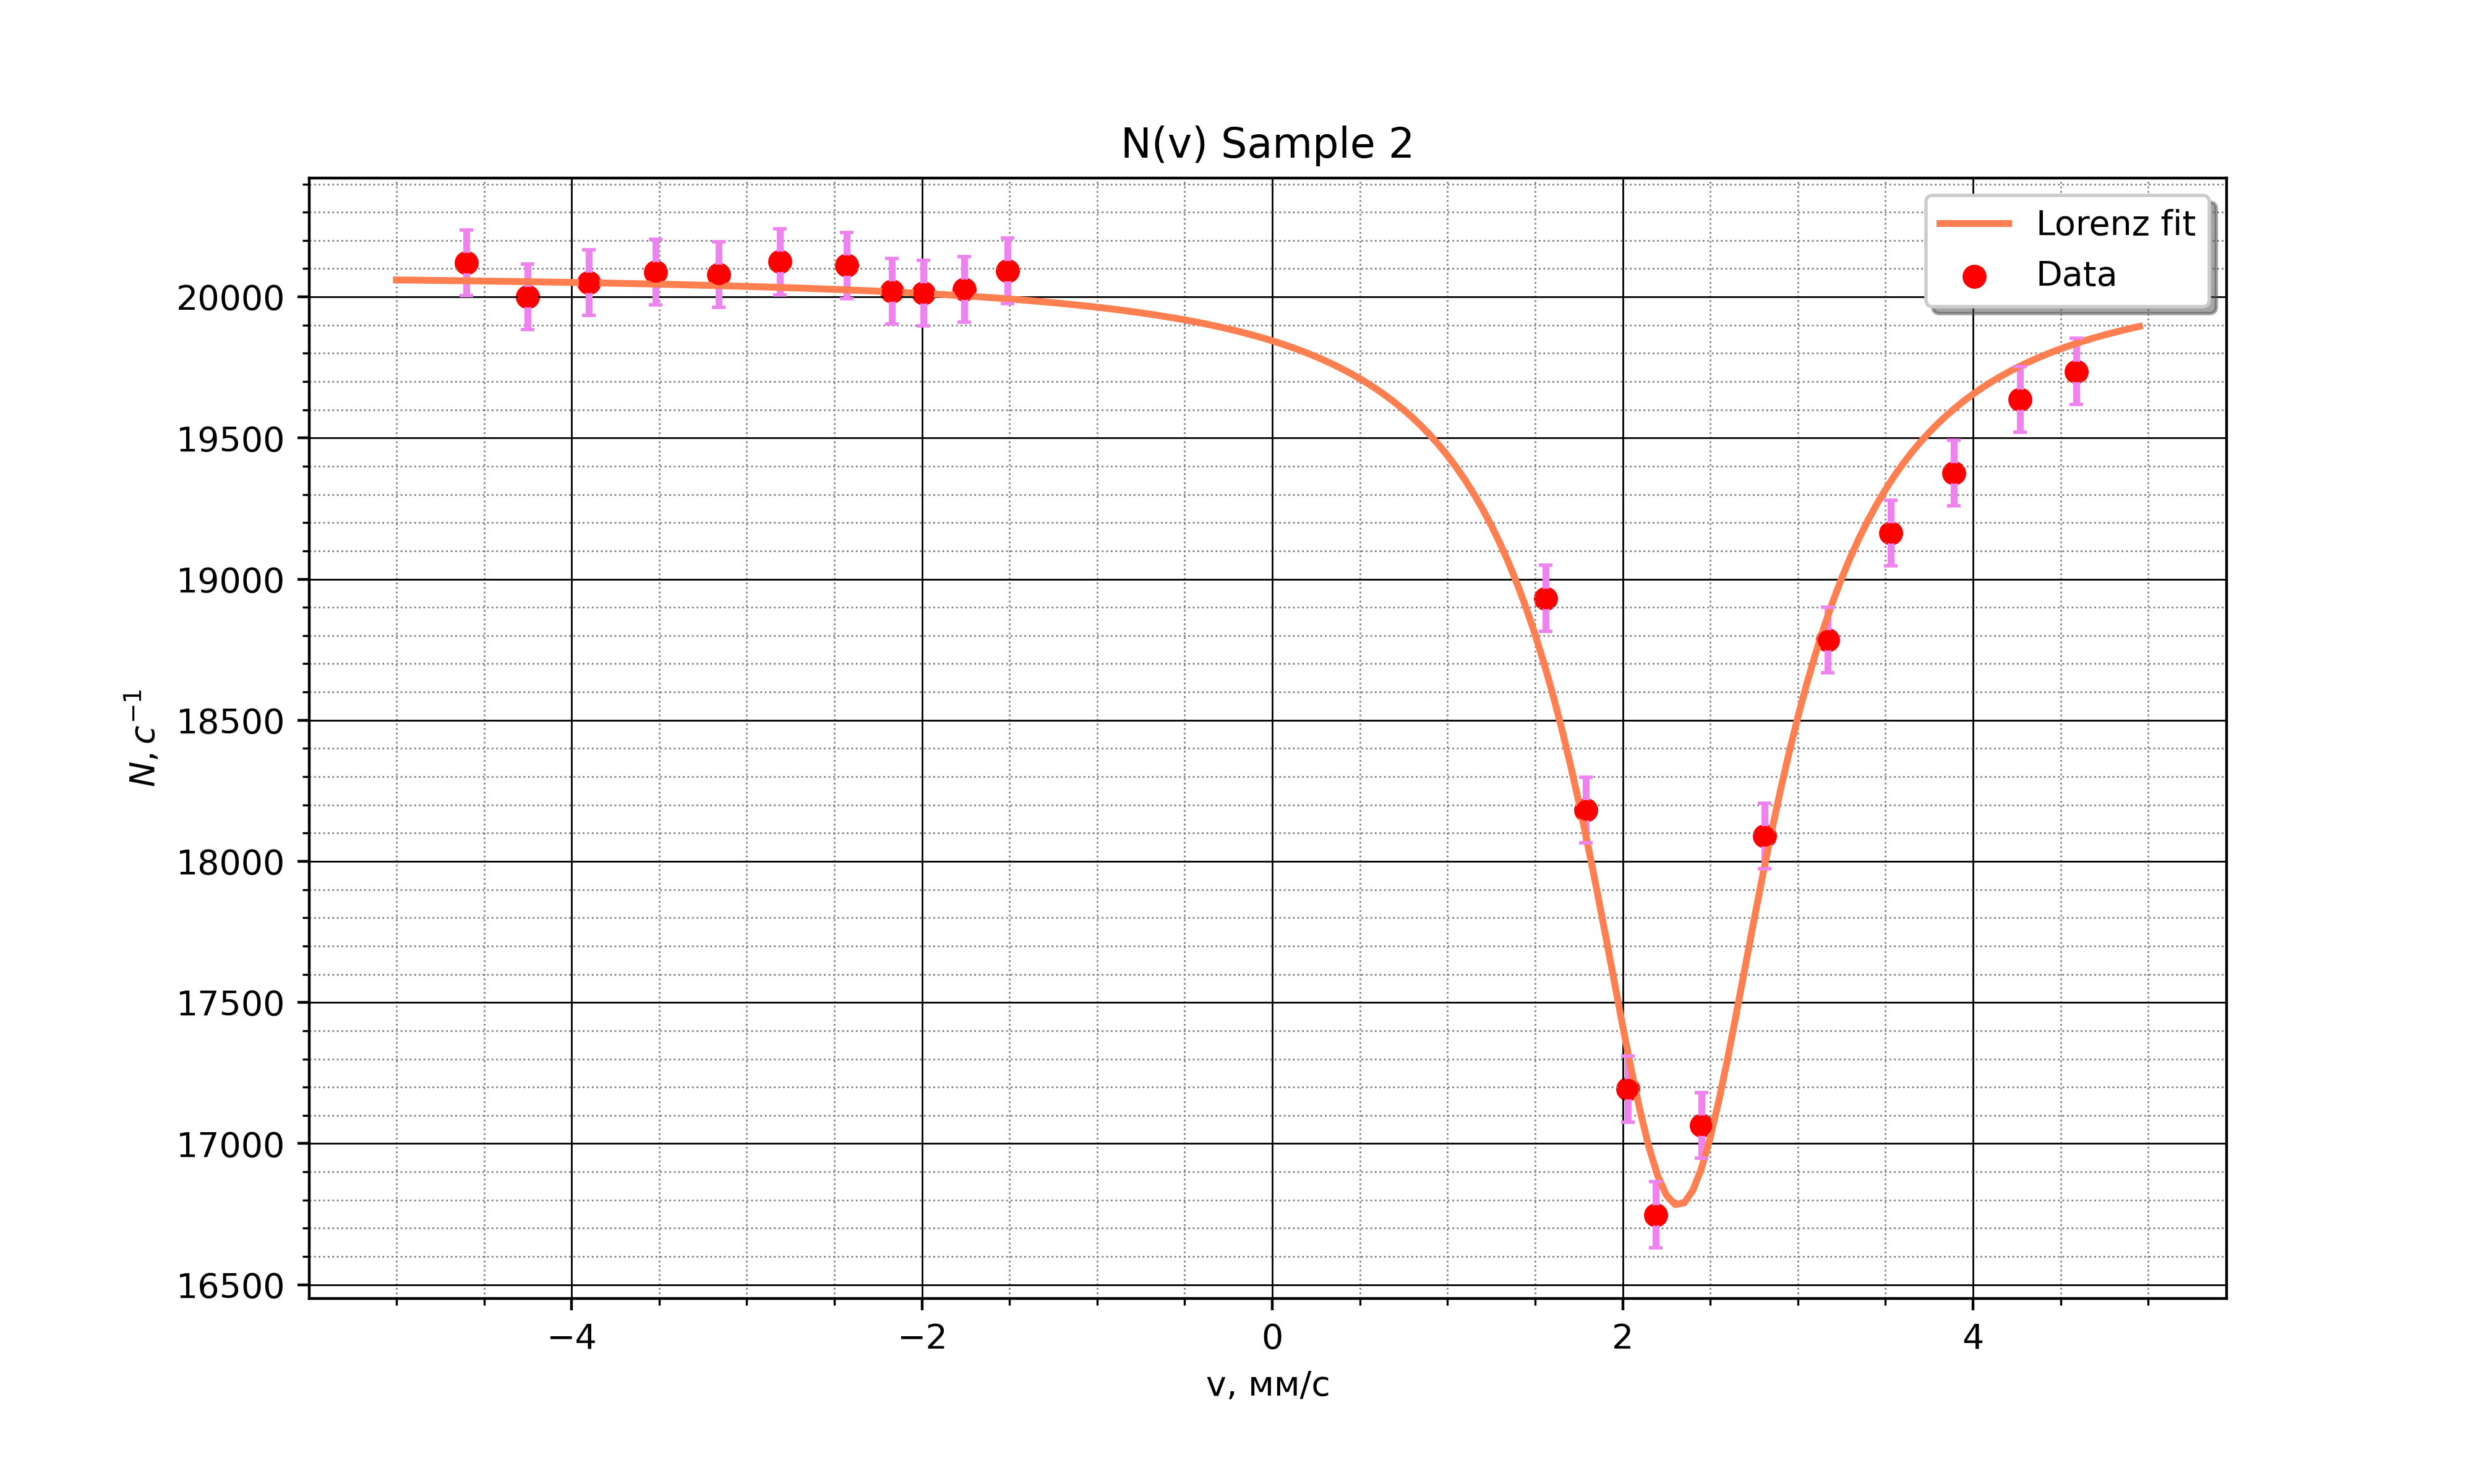
\includegraphics[scale = 0.5]{S2fit.png}
        \caption{Резонансное поглощение на 2-м образце}
        \label{S2fit}
    \end{center}
\end{figure}

\begin{figure}[H]
    \begin{center}
        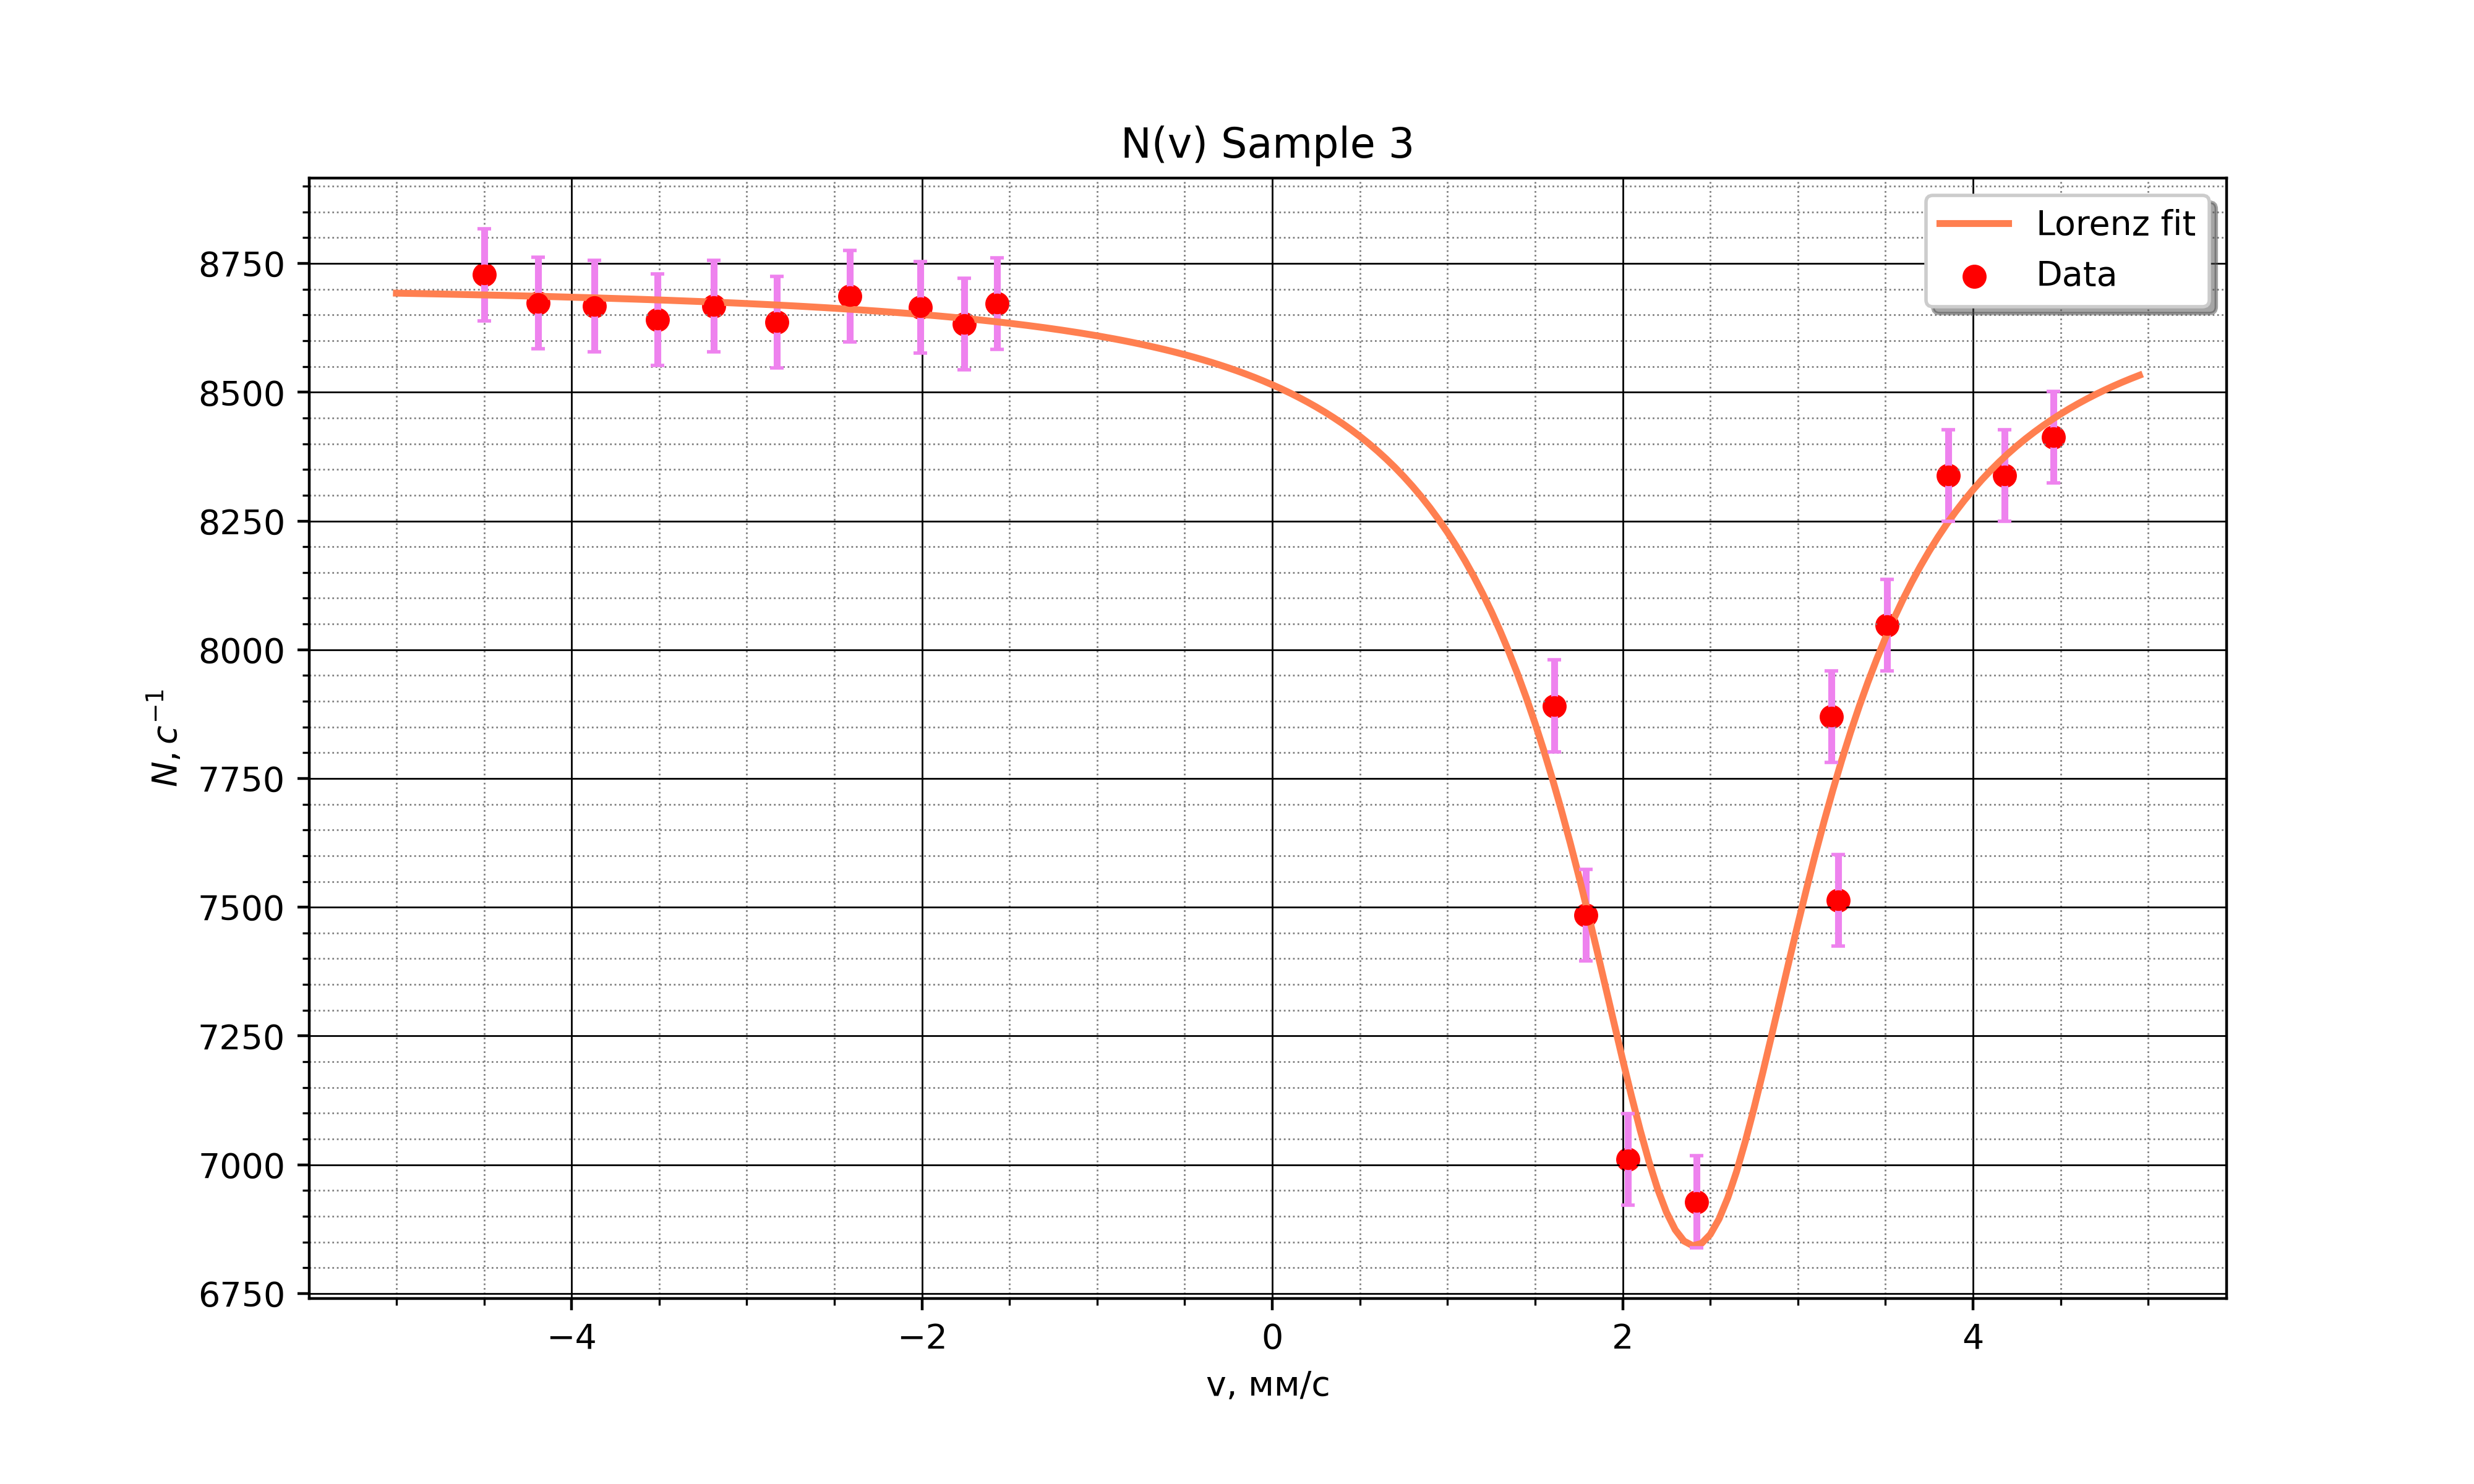
\includegraphics[scale = 0.5]{S3fit.png}
        \caption{Резонансное поглощение на 3-м образце}
        \label{S3fit}
    \end{center}
\end{figure}

\begin{figure}[H]
    \begin{center}
        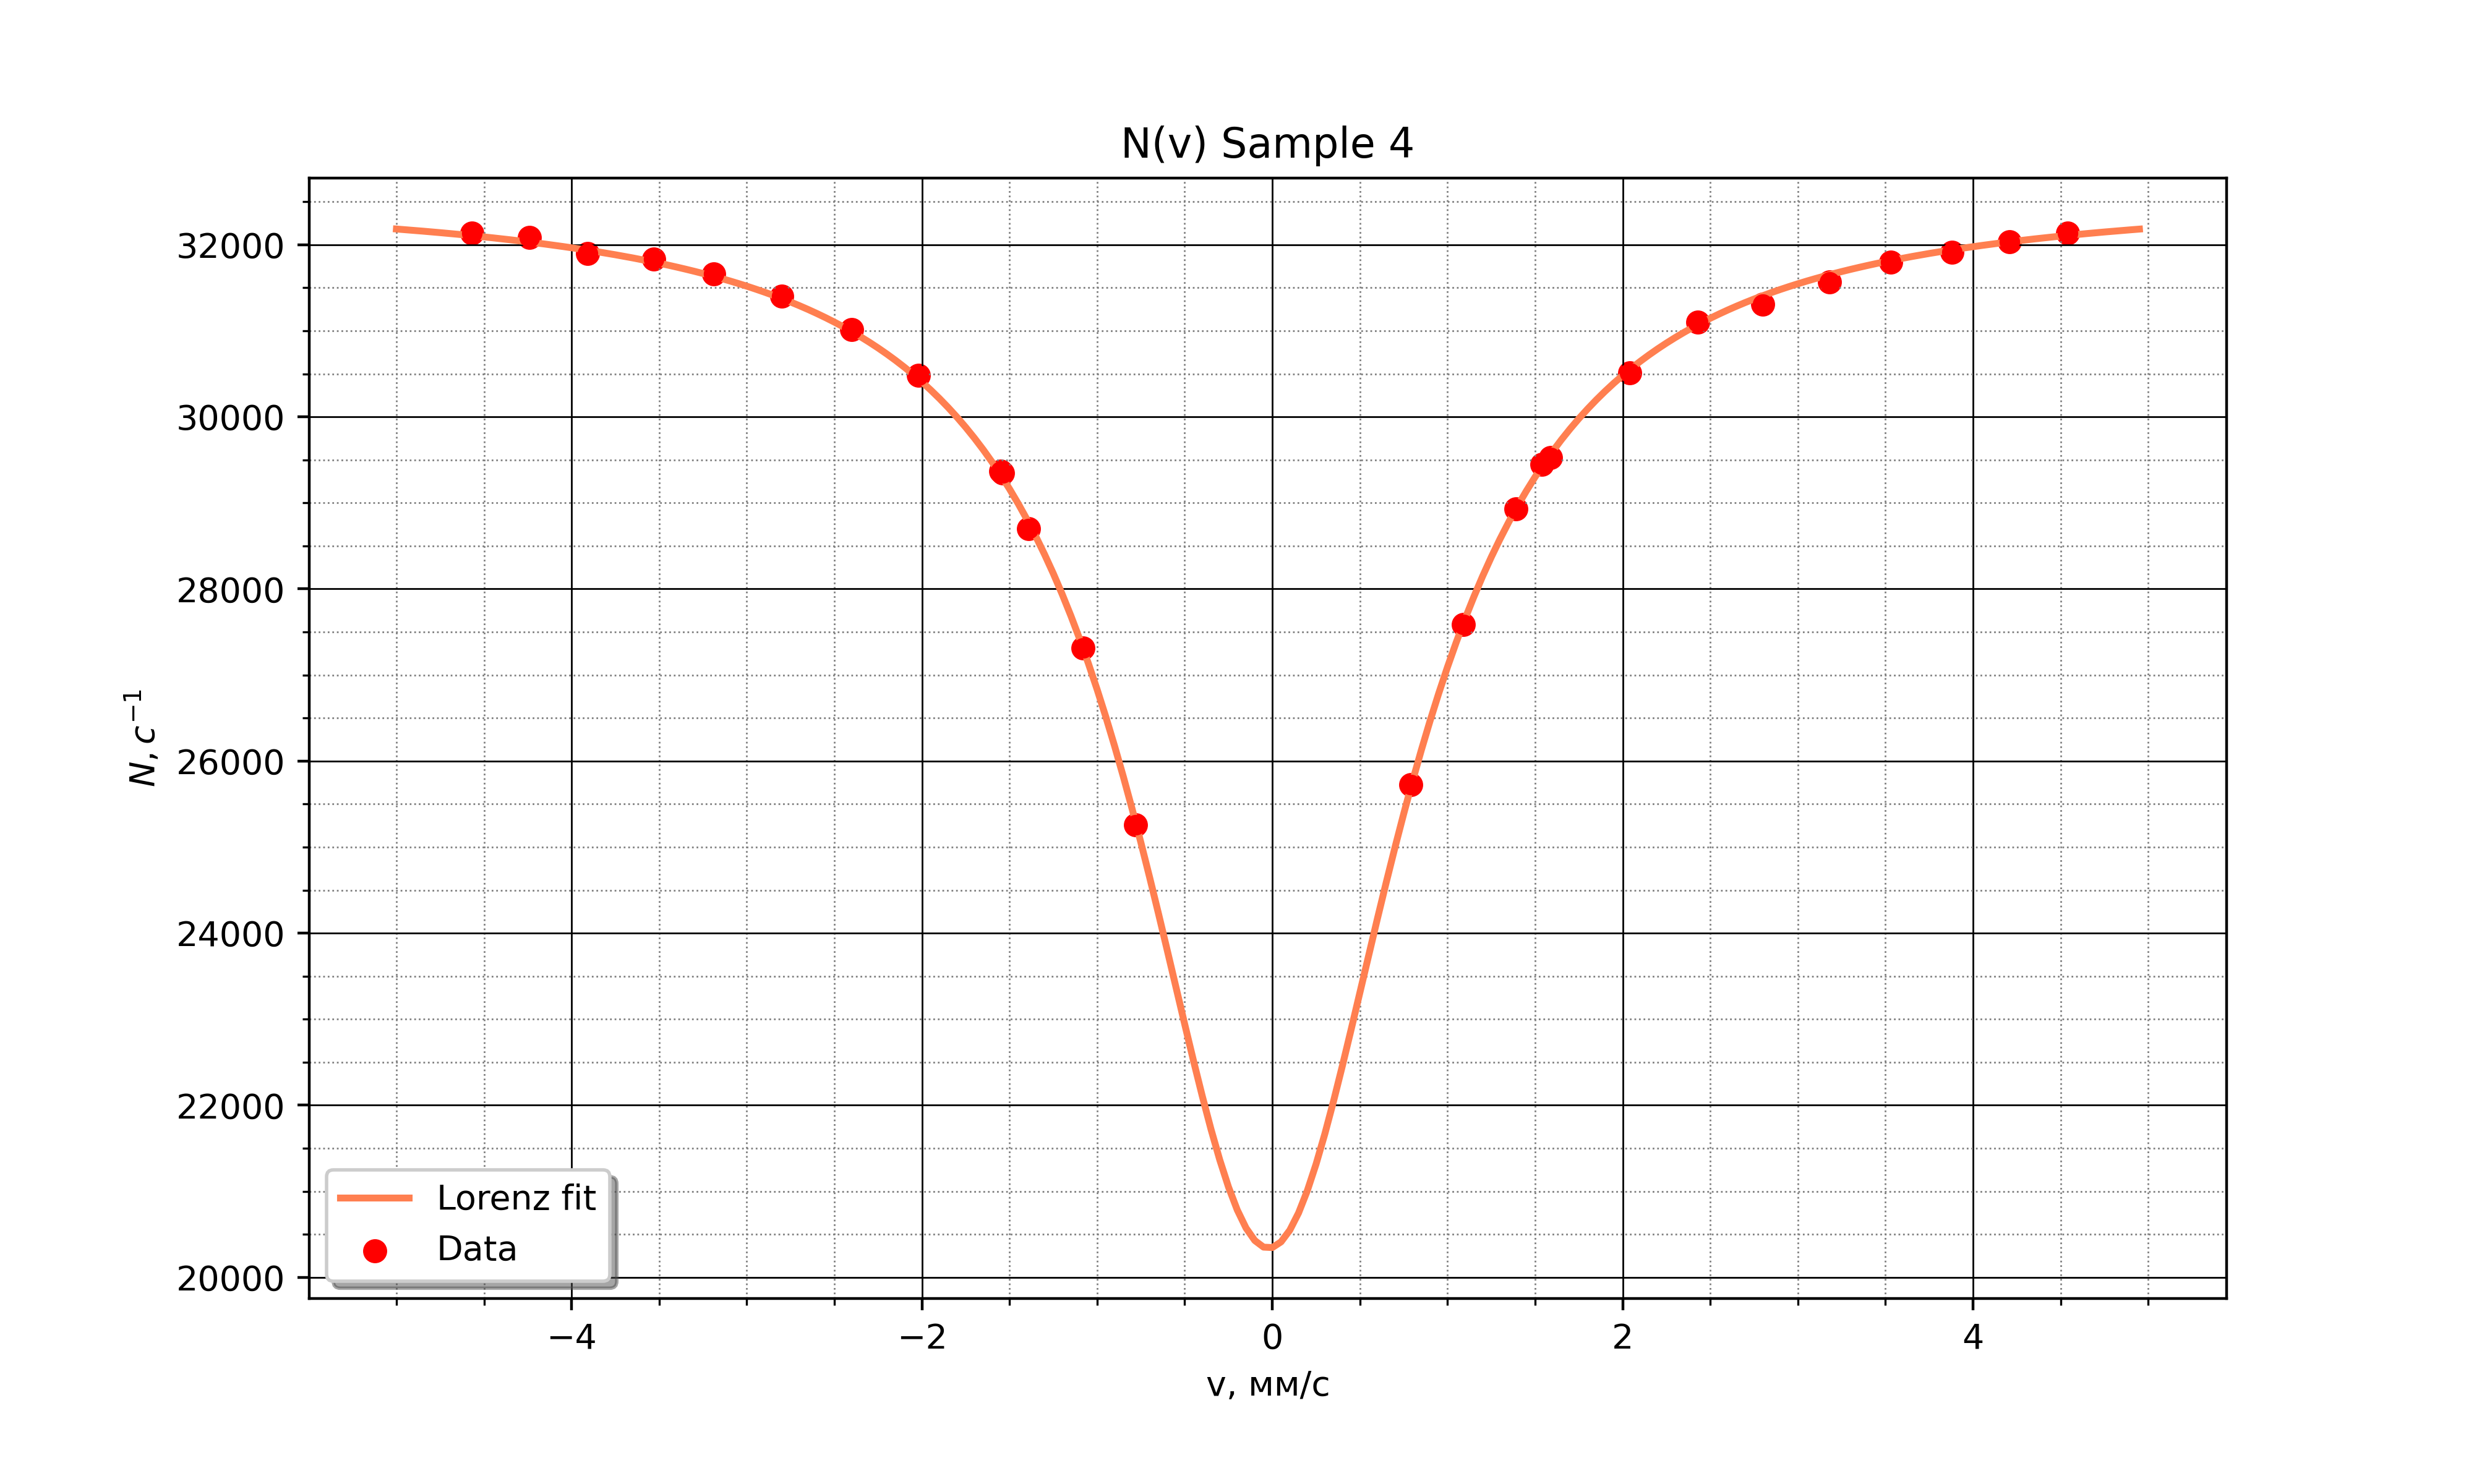
\includegraphics[scale = 0.5]{S4fit.png}
        \caption{Резонансное поглощение на 4-м образце}
        \label{S4fit}
    \end{center}
\end{figure}

\begin{figure}[H]
    \begin{center}
        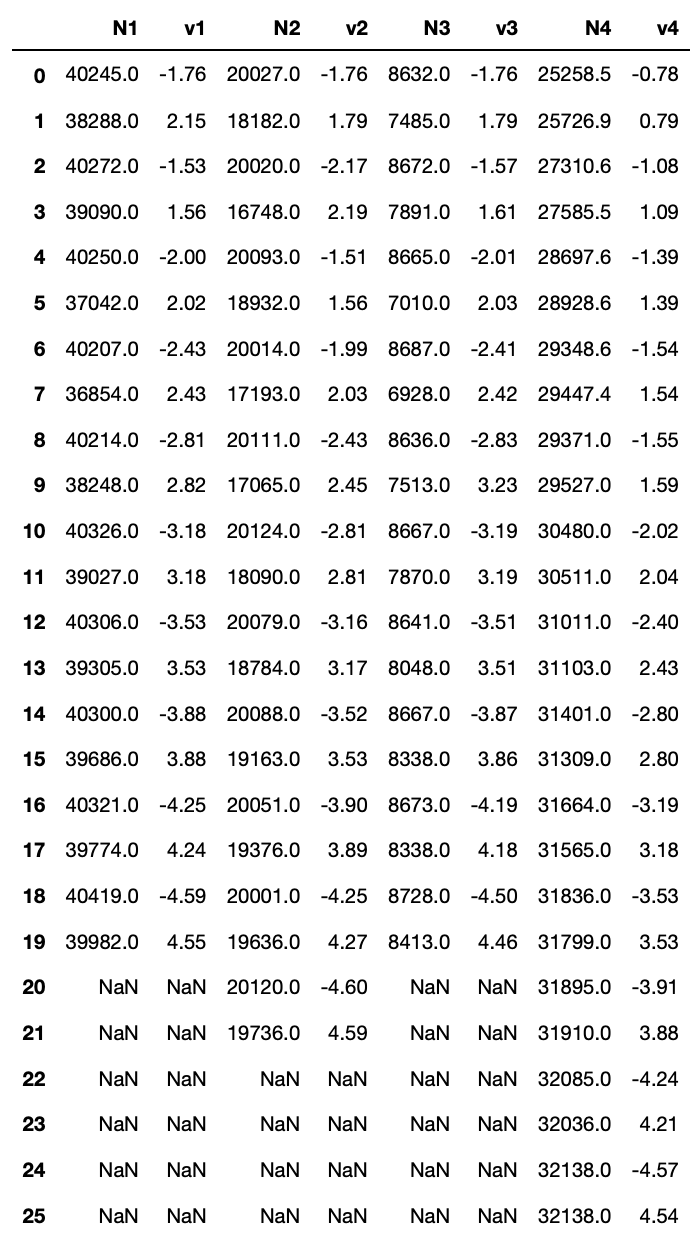
\includegraphics[scale = 0.5]{data.png}
        \caption{Общие данные поглощения}
        \label{data}
    \end{center}
\end{figure}




\end{document}